\documentclass[11pt, oneside]{article}
\usepackage[margin=1in,letterpaper]{geometry}
\usepackage{times}
\usepackage{graphicx}
\usepackage{amssymb,amsmath}
\usepackage{array}
\usepackage{longtable}
\usepackage{color}
\usepackage[T1]{fontenc}
\usepackage{sectsty}
\usepackage{tikz}
\usetikzlibrary{decorations.markings,calc,patterns}
\usepackage{pgfplots}
\pgfplotsset{compat=1.17}
\sectionfont{\fontsize{12}{12}\selectfont}
\subsectionfont{\fontsize{11}{11}\selectfont}
\subsubsectionfont{\normalsize\itshape\mdseries}

\renewcommand\labelitemi{{\boldmath$\cdot$}}

%%%%%%%%%%%%%%%%%%%%%%%%%%%%%%%%%%%%%
% Notation: vectors are bold (handwritten: underlined); unit vectors are \hat{\mathbf{x}}, etc.
% Per the master table: lowercase wavenumbers k, k_x, k_y (D14; handwritten K, K_x, K_y), power densities in script
% \mathcal{S} (D10; handwritten S_s, S_r), and the unit normal \hat{a} (handwritten \hat{n}), as in Lectures 4--6.
% Symbols kept as handwritten but flagged as pending dual usages in the master table (D45--D61): radar cross section
% sigma and backscattering coefficient sigma^0 (sigma is conductivity from L1); the surface-height autocorrelation
% function rho(r) (rho is reserved for Fresnel coefficients); rms height h (also plate separation, L1, and the h-pol
% subscript); correlation length ell (L4 loop length); characteristic slope m (mass, L1); surface height xi(x,y)
% (displacement, L1/L4); polarization indices p, q; the transmit/receive labels t, r (reflected/transmitted in L4--L5);
% the distances r_t, r_r, r and lag r; spectral wavenumbers k_x, k_y; lags u, v; the "scattered" label s; primes for
% local angles; f_a; the scatterer index i in sigma_i, A_i; the scattering azimuth phi_s; lambda_surf.
% Main textbook checks: Ulaby & Long (2014), Secs. 3-2, 5-4, 5-5, 5-10, 10-2, 10-3; van Zyl (2011), Secs. 1.3, 5.1, 5.2.
%%%%%%%%%%%%%%%%%%%%%%%%%%%%%%%%%%%%%

\title{Ge 158 Lecture 7: Scattering from Nonplanar Surfaces}
\author{Brent Minchew}
\date{}

\begin{document}
\maketitle

\noindent\textbf{Topics covered}
\begin{itemize}
	\item Radar equation
	\item Simple analytical models for scattering from rough surfaces
	\item Geometric properties of rough surfaces
	\item Scattering from undulating surfaces
\end{itemize}

%%%%%%%%%%%%%%%%%%%%%%%%%%%%%%%%%%%%%
% NOTE (notation, instructor decisions 2026-09-29, master table D46, D49, D52, D53, D59, D61): range r -> R (R_t, R_r);
% receive areas A_r, A_rs -> A_eff, A_eff,s; scatterer index i -> (n); correlation function rho(r) -> C(r) (script);
% slope parameter m -> m_s; surface wavelength lambda_surf -> Lambda (lambda_EM -> lambda).
\section{Models for microwave backscattering from rough surfaces}

\subsection{Motivation}

Motivation for focusing on microwave scattering:
\begin{itemize}
	\item reinforce and expand on basic concepts discussed already;
	\item useful for SAR observations;
	\item sets up discussions of volume scattering and radiometry, which we'll discuss in the next few classes.
\end{itemize}

\subsection{The radar equation}
\label{s:radar}

\begin{itemize}
	\item Let's build more intuition for how we actually measure and quantify scattering.
	\item This is a heuristic model known as the ``radar equation.'' Key components:
	\begin{enumerate}
		\item transmit power from the antenna;
		\item radiated power from the target (``scatterer'');
		\item effects of geometry, particularly \underline{spreading}.
	\end{enumerate}
\end{itemize}

\begin{figure}[!htbp]
	\centering
	% NOTE: sketch of the components of the radar equation, added at the instructor's request (not in the handwriting),
	% after the schematic whatissar01.gif, with symbols as in this lecture and the master table. Transmitter at upper left, receiver at upper right, scatterer on the ground.
	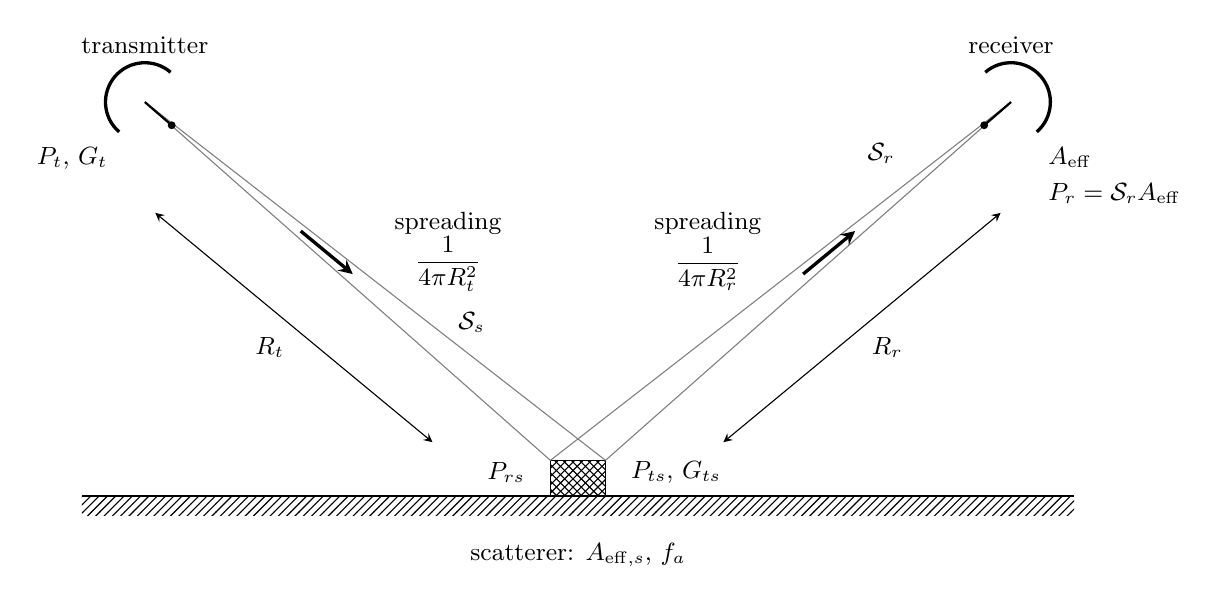
\begin{tikzpicture}[>=stealth, font=\small]
		\coordinate (tx) at (0,5);
		\coordinate (rx) at (11,5);
		\coordinate (sc) at (5.5,0.45);
		% ground
		\draw[thick] (-0.8,0) -- (11.8,0);
		\fill[pattern=north east lines] (-0.8,0) rectangle (11.8,-0.25);
		% scatterer
		\fill[pattern=crosshatch] (5.15,0) rectangle (5.85,0.45);
		\draw (5.15,0) rectangle (5.85,0.45);
		% transmit and receive beams
		\draw[gray] (tx) -- (5.15,0.45);
		\draw[gray] (tx) -- (5.85,0.45);
		\draw[gray] (5.15,0.45) -- (rx);
		\draw[gray] (5.85,0.45) -- (rx);
		% antennas (dishes facing the scatterer)
		\foreach \p/\d in {tx/-40.8, rx/220.8} {
			\draw[very thick] ($(\p)+(\d+90:0.5)$) arc[start angle=\d+90, end angle=\d+270, radius=0.5];
			\draw[thick] (\p) -- ($(\p)+(\d:0.45)$);
			\fill ($(\p)+(\d:0.45)$) circle (0.05);
		}
		\node[above=14pt] at (tx) {transmitter};
		\node[above=14pt] at (rx) {receiver};
		\node[anchor=north east, align=right] at ($(tx)+(-0.35,-0.45)$) {$P_t$, $G_t$};
		\node[anchor=north west, align=left] at ($(rx)+(0.35,-0.45)$) {$A_\mathrm{eff}$\\[2pt]$P_r = \mathcal{S}_r A_\mathrm{eff}$};
		% direction-of-travel arrows
		\draw[->, very thick] ($(tx)!0.36!(sc)$) -- ($(tx)!0.48!(sc)$);
		\draw[->, very thick] ($(sc)!0.52!(rx)$) -- ($(sc)!0.64!(rx)$);
		% ranges (offset perpendicular to the beams, on the outside)
		\coordinate (ta) at ($(tx)!1.0cm!-90:(sc)$); \coordinate (tb) at ($(sc)!1.0cm!90:(tx)$);
		\draw[<->] ($(ta)!0.14!(tb)$) -- node[below left=0pt] {$R_t$} ($(ta)!0.78!(tb)$);
		\coordinate (ra) at ($(rx)!1.0cm!90:(sc)$); \coordinate (rb) at ($(sc)!1.0cm!-90:(rx)$);
		\draw[<->] ($(ra)!0.14!(rb)$) -- node[below right=0pt] {$R_r$} ($(ra)!0.78!(rb)$);
		% spreading (inside the V)
		\node[align=center] at (3.85,3.1) {spreading\\$\dfrac{1}{4\pi R_t^2}$};
		\node[align=center] at (7.15,3.1) {spreading\\$\dfrac{1}{4\pi R_r^2}$};
		% power densities near the scatterer and receiver
		\node at (4.15,2.2) {$\mathcal{S}_s$};
		\node at (9.35,4.35) {$\mathcal{S}_r$};
		% scatterer properties
		\node[align=center] at (5.5,-0.75) {scatterer: $A_{\mathrm{eff},s}$, $f_a$};
		\node[anchor=east] at (4.95,0.3) {$P_{rs}$};
		\node[anchor=west] at (6.05,0.3) {$P_{ts}$, $G_{ts}$};
	\end{tikzpicture}
	\caption{Components of the radar equation (Section~\ref{s:radar}). The transmitter radiates power $P_t$ with gain $G_t$; the power density spreads as $1/(4\pi R_t^2)$, giving $\mathcal{S}_s$ at the scatterer. The scatterer intercepts $P_{rs} = \mathcal{S}_sA_{\mathrm{eff},s}$, absorbs a fraction $f_a$, and reradiates $P_{ts} = P_{rs}(1 - f_a)$ with gain $G_{ts}$ toward the receiver; after spreading as $1/(4\pi R_r^2)$, the power density $\mathcal{S}_r$ at the receiver gives the received power $P_r = \mathcal{S}_rA_\mathrm{eff}$.}
	\label{f:radar}
\end{figure}

These components are sketched in Figure~\ref{f:radar}.
% NOTE: added the pointer sentence to the new Figure f:radar.

\subsubsection{Spreading}

% NOTE: handwritten reads "power density (W/m^2) drops off as r^2"; written "as 1/r^2" (the power density is inversely
% proportional to the area 4 pi r^2 of the sphere; U&L 2014, Eq. 3.33, p. 85).
\begin{itemize}
	\item[$\hookrightarrow$] Spreading comes from the fact that radiated energy spreads as a sphere
	\begin{itemize}
		\item[$\Rightarrow$] the power density (W/m$^2$) % NOTE: handwritten "R^2 -> surface area of sphere with radius R"; the arrow is a pointer, not a limit, so written as a
		% parenthetical; added "4 pi".
		drops off as $1/R^2$ ($4\pi R^2$ is the surface area of a sphere with radius $R$).
	\end{itemize}
	% NOTE: added "(and, for a source of largest dimension d_ant, r >= 2 d_ant^2/lambda)": U&L 2014, Eq. 3.1 (p. 77), define the
	% far-field distance by a maximum phase error pi/8 between the spherical wave and its plane-wave approximation.
	\item[$\hookrightarrow$] This is consistent with the plane-wave assumption that we have been making, because the curvature of the sphere is negligible in the ``far field,'' where $R \gg \lambda$ (wavelength) (and, for a source of largest dimension $d_\mathrm{ant}$, $R \ge 2d_\mathrm{ant}^2/\lambda$).
\end{itemize}

\subsubsection{From the antenna to the scatterer}

\begin{itemize}
	\item Let's start from the source.
	% NOTE: handwritten reads "This has power per unit solid angle at the antenna = P_t G_t"; corrected to P_t G_t/(4 pi):
	% an isotropic antenna spreads P_t over 4 pi sr, and the gain multiplies this (U&L 2014, Eq. 3.23, p. 84, gives
	% R^2 S_max = P_t G/(4 pi); Eq. 5.26, p. 170). The product P_t G_t is the power an isotropic antenna would need to
	% transmit to give the same power density (added sentence; cf. U&L p. 170, van Zyl 2011, Fig. 1-6, p. 10). Also added
	% "(in the direction of the scatterer)"; "at the antenna" is as handwritten.
	\item Consider an antenna with transmit power $P_t$ and gain $G_t$. This has power per unit solid angle at the antenna (in the direction of the scatterer) $= P_tG_t/(4\pi)$; $P_tG_t$ is the power that an isotropic antenna would have to transmit to produce the same power density.
	\item At the scatterer, a distance $R_t$ from the antenna, we need to take into account the reduction of power density due to spreading. So, the power density at the scatterer (magnitude of the Poynting vector) is
	% NOTE: handwritten S_s is written \mathcal{S}_s (script, master table D10). Checked against U&L 2014, Eq. 5.26
	% (p. 170) and van Zyl 2011, Fig. 1-6 (p. 10).
	\begin{equation}
		\label{e:Ss}
		\mathcal{S}_s = \left[P_tG_t\right]\left(\frac{1}{4\pi R_t^2}\right),
		\qquad
		\frac{\text{power}}{\text{area}} = \left[\begin{array}{c}\text{power transmitted}\\ \text{from antenna}\end{array}\right]\left(\begin{array}{c}\text{spreading}\\ \text{losses}\end{array}\right).
	\end{equation}
	\item The total power received by the scatterer, $P_{rs}$, must account for the effective receiving area of the scatterer, $A_{\mathrm{eff},s}$:
	\begin{equation}
		\label{e:Prs}
		\Rightarrow\quad P_{rs} = \mathcal{S}_sA_{\mathrm{eff},s}.
	\end{equation}
	\item[$\bigstar$] Note: $A_{\mathrm{eff},s}$ is \underline{not} the area illuminated by the incident beam but rather an unknown property of the scatterer.
\end{itemize}

\subsubsection{From the scatterer to the receiver}

\begin{itemize}
	\item Some power will be absorbed by the scatterer; the rest will be radiated in various directions. The power radiated by the scatterer is
	\begin{equation}
		\label{e:Pts}
		P_{ts} = P_{rs}\left(1 - f_a\right),
	\end{equation}
	where $f_a \equiv$ fraction of power absorbed by the scatterer.
	\item Incident radiation will induce currents (free currents and bound currents due to conductivity and electric displacement $\rightarrow$ i.e., the non-magnetic terms in Amp\`ere's law)
	\begin{itemize}
		\item[$\Rightarrow$] we can treat the scatterer as an antenna:
		\begin{equation}
			\label{e:Sr}
			\mathcal{S}_r = \frac{P_{ts}G_{ts}}{4\pi R_r^2},
		\end{equation}
		where
		\begin{itemize}
			\item $G_{ts} \equiv$ gain of the scatterer in the direction of the receiver;
			\item $R_r \equiv$ distance from the scatterer to the receiver.
		\end{itemize}
	\end{itemize}
	\item Finally, the power entering the receiver is a function of the effective area of the aperture, $A_\mathrm{eff}$ (not necessarily the physical size of the aperture):
	\begin{equation}
		\label{e:Pr}
		P_r = \mathcal{S}_rA_\mathrm{eff}.
	\end{equation}
\end{itemize}

\subsubsection{Radar cross section}

% NOTE: checked by substituting Eqs. (e:Ss)--(e:Pr) (by hand and python3) and against U&L 2014, Eqs. 5.27a--5.28b
% (p. 170), where U&L's sigma_pq plays the role of A_rs (1 - f_a) G_ts and xi_r A_r that of A_r.
\begin{itemize}
	\item Putting it all together, we can write an expression for the received power:
	\begin{equation}
		\label{e:radar}
		P_r = \underbrace{\left(\frac{P_tG_tA_\mathrm{eff}}{\left(4\pi\right)^2R_t^2R_r^2}\right)}_{\text{knowns}}\underbrace{\left[A_{\mathrm{eff},s}\left(1 - f_a\right)G_{ts}\right]}_{\text{unknowns}}.
	\end{equation}
	\item In general, the bracketed term is unknown and is a term of interest. Let us define it as
	\begin{equation}
		\label{e:rcs}
		\sigma = A_{\mathrm{eff},s}\left(1 - f_a\right)G_{ts} \qquad [\text{units: m}^2]
	\end{equation}
	and call it the \emph{radar (scattering) cross section}, as it has units of m$^2$. (Note: in this class, I have tried to use variables in a way that is consistent with usage in RS, and here we have encountered one of the unfortunate inconsistencies in conventional variables, with $\sigma$ now being used to denote something other than electrical conductivity.)
	% NOTE: U&L 2014, Eq. 5.33a (p. 171): sigma^0 = sigma/A for a distributed target of horizontal area A.
	\item More commonly, we normalize by the nominal area of illumination to get the normalized radar cross section (``sigma-naught''):
	\begin{equation}
		\label{e:sigma0}
		\sigma^0 = \left\langle\frac{\sigma_{(n)}}{A_{(n)}}\right\rangle_n,
	\end{equation}
	where $\sigma_{(n)} \equiv$ radar cross section for an individual scatterer and $\langle\cdot\rangle$ denotes the spatial average.
\end{itemize}

\subsubsection{Accounting for polarization}

\begin{itemize}
	\item Up to this point, we have ignored wave polarization for simplicity. We can account for polarization by noting that the transmitted and received powers are polarization dependent:
	\begin{itemize}
		\item $P_p^r \equiv$ $p$-polarized received power (horizontal or vertical);
		\item $P_q^t \equiv$ $q$-polarized transmit power ($h$ or $v$).
	\end{itemize}
	% NOTE: checked against U&L 2014, Eq. 5.32 (p. 171; they write R_a for r and G(theta_a, phi_a) for the gain in the
	% direction of each element dA), and by substitution into Eq. (e:radar) (python3).
	\begin{equation}
		\label{e:radar_pol}
		P_p^r = \frac{\lambda^2}{\left(4\pi\right)^3}\int_{\substack{\text{area}\\ \text{illuminated}}}\frac{P_q^tG^2}{R^4}\,\sigma_{pq}^0\,dA,
	\end{equation}
	where we have assumed
	\begin{equation}
		G_r = G_t = G \qquad \text{and} \qquad R_t = R_r = R
	\end{equation}
	% NOTE: added "(for a lossless antenna)". In general A_r = (lambda^2/4 pi) D_r and G_r = xi_r D_r (U&L 2014,
	% Eqs. 3.24 and 3.31b, pp. 84--85), so lambda^2 G_r/(4 pi) = xi_r A_r, which equals A_r only when the radiation
	% efficiency xi_r = 1 (U&L Eq. 5.28b, p. 170).
	and applied the identity (for a lossless antenna)
	\begin{equation}
		\label{e:Ae}
		A_\mathrm{eff} = \frac{\lambda^2G_r}{4\pi}.
	\end{equation}
	% NOTE: added "$E_q^i$ is the incident electric field" (the handwriting labels only E_p^s, "scattered electric field").
	% NOTE: added "measured in the far field of the scatterer": U&L 2014, Eqs. 5.30 (p. 171) and 5.114 (p. 200), define
	% sigma through the limit R_r -> infinity, with S_p^s = |E_p^s|^2/(2 eta_0) and S_q^i = |E_q^i|^2/(2 eta_0).
	\item For intuition, we can note that
	\begin{equation}
		\label{e:sigma0_field}
		\sigma_{pq}^0 = \frac{4\pi R^2}{A}\,\frac{|E_p^s|^2}{|E_q^i|^2} = \frac{4\pi R^2}{A}\,\Gamma_{pq},
	\end{equation}
	where $E_p^s$ is the scattered electric field (measured in the far field of the scatterer), $E_q^i$ is the incident electric field, and $\Gamma_{pq}$ is the reflectance, a generalization of the reflectance we derived before for planar surfaces (Lecture 5).
	% NOTE: added the following sentence at the instructor's request (master table D63).
	Unlike the reflectivity $\Gamma = |\rho|^2$ of an infinite planar interface (Lectures 4--5), $\Gamma_{pq}$ depends on the range $R$ at which the scattered field is measured: the field scattered by the finite illuminated area $A$ spreads spherically, so $|E_p^s|^2 \propto 1/R^2$. The factor $4\pi R^2/A$ in Eq.~\eqref{e:sigma0_field} removes this dependence, which makes $\sigma_{pq}^0$ a property of the surface alone.
	% NOTE: added "(Lecture 5)".
\end{itemize}

%%%%%%%%%%%%%%%%%%%%%%%%%%%%%%%%%%%%%
\section{Scattering from nonplanar surfaces}
\label{s:nonplanar}

\subsection{Simple analytical models}

\begin{itemize}
	\item Now that we have a basic sense of how we often quantify the scattering of EM waves, let's consider some simple models for surfaces.
	\item We'll focus on simple analytical models.
	\item Simple analytical models only exist for a few special cases that occur when the spatial dimensions of the surface roughness are much smaller or much larger than the EM wavelength.
	\begin{itemize}
		% NOTE: handwritten cites "Fung (1992, 2002)"; written "Fung et al. (1992, 2002)" (Fung, Li & Chen 1992;
		% Fung, Liu, Chen & Tsay 2002; U&L 2014, p. 428 and bibliography).
		\item[$\hookrightarrow$] For the intermediate case, when roughness $\sim$ EM wavelength, very complex models are necessary. We won't go over these in class because they offer little additional insight. But one such model, known as the Integral Equation Model (IEM), is discussed in Ulaby and Long (2014), Chapter 10, and in the primary literature, Fung et al.\ (1992, 2002), for those who are interested.
	\end{itemize}
\end{itemize}

\subsection{Basic concepts of surface scattering}

\begin{itemize}
	\item For surface scattering, we are concerned with
	\begin{itemize}
		\item the total power reflected by the surface (reflectivity);
		\item the direction of scattering.
	\end{itemize}
	\item Scattering from an area is simply (re)radiation from the area $\Rightarrow$ many concepts discussed here are adopted from antenna theory (which we will not discuss in detail, but those interested in learning more can consult Ulaby and Long (2014), Ch.~3).
	% NOTE: added "(Figure~\ref{f:roughness})".
	\item Key to understanding the direction of scatter is the surface roughness (Figure~\ref{f:roughness}).
\end{itemize}

\begin{figure}[h]
	\centering
	% Elements follow the handwritten sketch: three panels with z (up) and x axes (z extending below x); labels
	% "perfectly smooth" (left) and "perfectly rough" (right); incident unit vector k_i (arrowhead at the origin in the
	% left panel, mid-ray in the middle and right panels); reflected k_r in the left and middle panels; angle arcs theta_i
	% (both sides of z in the left and middle panels, one arc from the incident ray to z in the right panel); a small
	% lobe of scattered arrows (middle) and a wide lobe of arrows in all upward directions (right); the handwritten
	% text beneath each panel. In the right panel the incident ray ends at the lobe (arrowhead there). Illustrative angle: theta_i = 33 deg.
	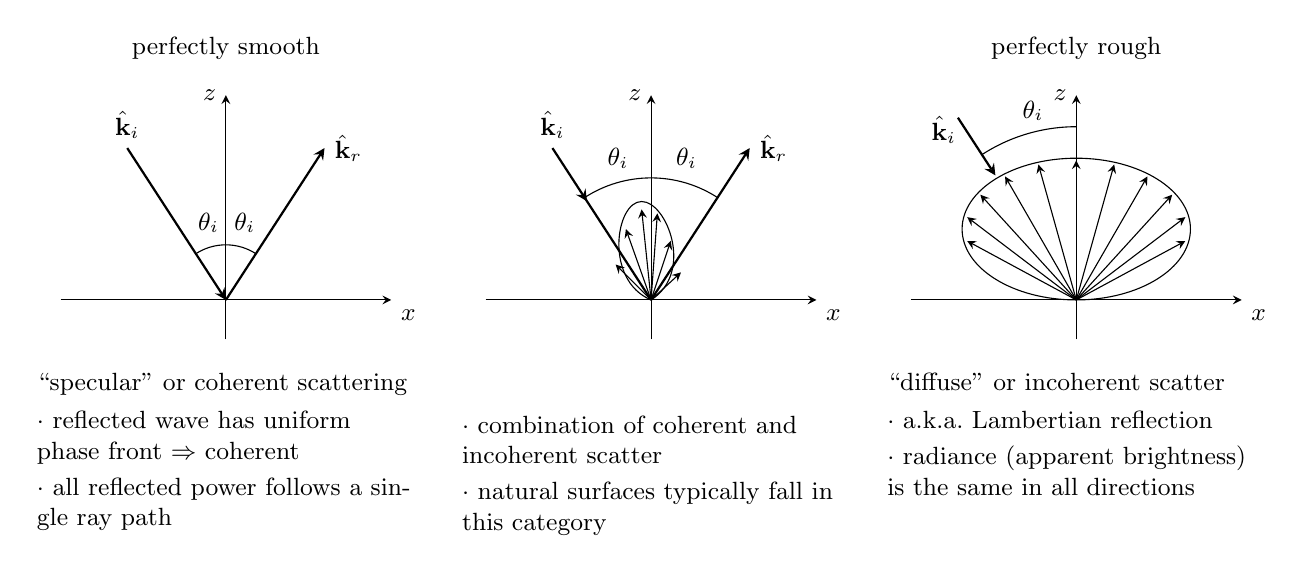
\begin{tikzpicture}[>=stealth, font=\small,
		mid/.style={postaction={decorate}, decoration={markings, mark=at position 0.35 with {\arrow{>}}}}]
		\def\ti{33}\def\L{2.3}
		\foreach \xs in {0, 5.4, 10.8} {
			\begin{scope}[xshift=\xs cm]
				\draw[->] (-2.1,0) -- (2.1,0) node[below right] {$x$};
				\draw[->] (0,-0.5) -- (0,2.6) node[left] {$z$};
			\end{scope}
		}
		% ---- left: perfectly smooth ----
		\node at (0,3.2) {perfectly smooth};
		\draw[->, thick] ({-\L*sin(\ti)},{\L*cos(\ti)}) -- (0,0);
		\node[above] at ({-\L*sin(\ti)},{\L*cos(\ti)}) {$\hat{\mathbf{k}}_i$};
		\draw[->, thick] (0,0) -- ({\L*sin(\ti)},{\L*cos(\ti)}) node[right] {$\hat{\mathbf{k}}_r$};
		\draw (0,0.7) arc (90:{90+\ti}:0.7);
		\draw (0,0.7) arc (90:{90-\ti}:0.7);
		\node at (-0.22,0.98) {$\theta_i$};
		\node at (0.24,0.98) {$\theta_i$};
		% ---- middle: combination ----
		\begin{scope}[xshift=5.4cm]
			\draw[thick, mid] ({-\L*sin(\ti)},{\L*cos(\ti)}) -- (0,0);
			\node[above] at ({-\L*sin(\ti)},{\L*cos(\ti)}) {$\hat{\mathbf{k}}_i$};
			\draw[->, thick] (0,0) -- ({\L*sin(\ti)},{\L*cos(\ti)}) node[right] {$\hat{\mathbf{k}}_r$};
			\draw (0,1.55) arc (90:{90+\ti}:1.55);
			\draw (0,1.55) arc (90:{90-\ti}:1.55);
			\node at (-0.42,1.8) {$\theta_i$};
			\node at (0.45,1.8) {$\theta_i$};
			\draw (0,0) .. controls (-0.6,0.25) and (-0.45,1.25) .. (-0.12,1.25) .. controls (0.2,1.25) and (0.55,0.35) .. (0,0);
			\foreach \px/\py in {-0.45/0.45, -0.32/0.9, -0.12/1.15, 0.08/1.1, 0.25/0.75, 0.38/0.35} \draw[->] (0,0) -- (\px,\py);
		\end{scope}
		% ---- right: perfectly rough ----
		\begin{scope}[xshift=10.8cm]
			\node at (0,3.2) {perfectly rough};
			\draw[->, thick] ({-1.2*\L*sin(\ti)},{1.2*\L*cos(\ti)}) -- ({-0.82*\L*sin(\ti)},{0.82*\L*cos(\ti)});
			\node[left] at ({-1.12*\L*sin(\ti)},{1.12*\L*cos(\ti)}) {$\hat{\mathbf{k}}_i$};
			\draw ({2.2*cos(90+\ti)},{2.2*sin(90+\ti)}) arc ({90+\ti}:90:2.2);
			\node at (-0.55,2.4) {$\theta_i$};
			\draw (0,0.9) ellipse (1.45 and 0.9);
			\foreach \t in {190,170,...,-10} \draw[->] (0,0) -- ({0.97*1.45*cos(\t)},{0.9+0.97*0.9*sin(\t)});
		\end{scope}
		% ---- text beneath the panels ----
		\node[anchor=north, text width=4.8cm, align=left] at (0,-0.8) {``specular'' or coherent scattering\\[3pt]
			$\cdot$ reflected wave has uniform phase front $\Rightarrow$ coherent\\[2pt]
			$\cdot$ all reflected power follows a single ray path};
		\node[anchor=north, text width=4.8cm, align=left] at (5.4,-1.35) {$\cdot$ combination of coherent and incoherent scatter\\[2pt]
			$\cdot$ natural surfaces typically fall in this category};
		\node[anchor=north, text width=4.8cm, align=left] at (10.8,-0.8) {``diffuse'' or incoherent scatter\\[3pt]
			$\cdot$ a.k.a.\ Lambertian reflection\\[2pt]
			$\cdot$ radiance (apparent brightness) is the same in all directions};
	\end{tikzpicture}
	\caption{Scattering patterns for a plane wave incident at angle $\theta_i$ on a perfectly smooth surface (left), a surface of intermediate roughness (middle), and a perfectly rough surface (right).}
	\label{f:roughness}
\end{figure}
% NOTE: the caption is an added description. Cf. U&L 2014, Fig. 5-30 (p. 197), and van Zyl 2011, pp. 197--198. The
% Lambertian statement agrees with U&L 2014, p. 253 (Eq. 6.108: scatters uniformly per unit projected area in all
% directions) and Liou (Sec. 7.3, p. 365: "Lambertian ... (isotropic reflection)").

\subsection{Characterizing surface roughness}

\begin{itemize}
	\item How do we define surface roughness? Two length scales:
	\begin{enumerate}
		\item RMS height $h$;
		\item correlation length $\ell$.
	\end{enumerate}
\end{itemize}

\subsubsection{Definitions}

% NOTE: the handwritten surface-height symbol reads as xi (low confidence; possibly zeta); xi as in van Zyl 2011,
% Eqs. 5.1-1 and 5.1-2 (p. 184), whose definitions (h, rho(r), l) these follow. U&L 2014 write z(x,y), s, rho(xi), l
% (Eqs. 5.103--5.106, pp. 194--196).
\begin{itemize}
	\item Let us define the local surface height as a 2D function $\xi(x,y)$.
	\item Assume $\xi$ has a Gaussian distribution with zero mean.
	\item Therefore, the RMS height is given by
	\begin{equation}
		\label{e:h}
		h^2 = \left\langle\xi^2(x,y)\right\rangle.
	\end{equation}
	\item But we need more information, specifically how the height at one point relates to the height at another point
	% NOTE: added "(for a statistically isotropic surface)": rho depends on the separation r alone only if the surface
	% statistics are isotropic (van Zyl 2011, p. 184; U&L 2014, p. 194).
	\begin{itemize}
		\item[$\Rightarrow$] auto-correlation function (for a statistically isotropic surface)
		\begin{equation}
			\label{e:acf}
			\mathcal{C}(r) = \frac{\left\langle\xi(x,y)\,\xi(x',y')\right\rangle}{h^2},
		\end{equation}
		where $r = \sqrt{(x - x')^2 + (y - y')^2}$ is the distance between the points.
	\end{itemize}
\end{itemize}

\subsubsection{Correlation functions}

% NOTE: checked against U&L 2014, Eqs. 5.107a,b (p. 196) and van Zyl 2011, Eqs. 5.1-3 and 5.1-4 (p. 184).
% Handwritten reads "l is distance over which correlation decreases by 1/e"; written "decreases to 1/e" (rho(l) = e^{-1};
% U&L 2014, Eq. 5.106, p. 196).
\begin{itemize}
	\item Two correlation functions are commonly assumed:
	\begin{itemize}
		\item Gaussian:
		\begin{equation}
			\label{e:acf_g}
			\mathcal{C}(r) = e^{-r^2/\ell^2};
		\end{equation}
		\item Exponential:
		\begin{equation}
			\label{e:acf_e}
			\mathcal{C}(r) = e^{-|r|/\ell}.
		\end{equation}
	\end{itemize}
	\item[$\Rightarrow$] This makes clear that $\ell$ is the distance over which the correlation decreases to $1/e$.
\end{itemize}

\subsubsection{Roughness spectrum}

\begin{itemize}
	\item It is more common to represent the surface in terms of the roughness spectrum
	\begin{equation}
		\label{e:W}
		W(k_x,k_y) = \frac{1}{2\pi}\int_{-\infty}^{\infty}\!\!\int_{-\infty}^{\infty}\mathcal{C}(u,v)\exp\left\{-j\left(k_xu + k_yv\right)\right\}du\,dv,
	\end{equation}
	% NOTE: handwritten reads "K_x = -K sin theta_s cos phi_s and K_y = K sin theta_s sin phi_s" (capital K; written k per
	% D14). Corrected k_x to k (sin theta_s cos phi_s - sin theta_i) because the spectral wavenumber that scatters into
	% (theta_s, phi_s) is the horizontal part of k_s - k_i (the phase of the field scattered from surface point (x,y) is
	% exp[j (k_s - k_i) . r], cf. the phase matching of Lecture 5), with the incident wave in the x-z plane. The handwritten
	% form fails two checks (python3): in the specular direction (theta_s = theta_i, phi_s = 0) it gives |k_x| = k sin
	% theta_i instead of 0 (a flat surface scatters only there), and in backscatter it gives k sin theta_i instead of the
	% Bragg value 2 k sin theta_i used by van Zyl 2011, Eqs. 5.2-4 and 5.2-7 (pp. 199--200: W(2k sin theta) and
	% W^n(-2k sin theta, 0)). W is even in k_x and k_y for an isotropic surface, so the overall sign is immaterial.
	% k is the wavenumber in the medium above the surface (k_0 for air). Added "with the incident wave in the x--z plane
	% propagating toward +x" and "from the forward, +x, direction" to fix the sign conventions.
	where
	\begin{equation}
		\label{e:kxky}
		k_x = k\left(\sin\theta_s\cos\phi_s - \sin\theta_i\right) \qquad \text{and} \qquad k_y = k\sin\theta_s\sin\phi_s,
	\end{equation}
	with the incident wave in the $x$--$z$ plane propagating toward $+x$, and where
	\begin{itemize}
		\item $\theta_s \equiv$ scattering angle;
		\item $\phi_s \equiv$ scattering azimuth (the angle between the plane of incidence and the propagation vector of the scattered wave, measured in the horizontal plane from the forward, $+x$, direction).
	\end{itemize}
	% NOTE: added the consequence "=> (k_x, k_y) = (-2k sin theta_i, 0)" (van Zyl 2011, Eq. 5.2-7, p. 200; U&L 2014, p. 196,
	% define backscatter as theta_s = theta_i, phi = 180 deg).
	\item Ex.: for the case where a signal is transmitted and received by the same antenna, $\theta_s = \theta_i$ and $\phi_s = \pi$ $\Rightarrow$ $(k_x, k_y) = (-2k\sin\theta_i, 0)$.
	% NOTE: checked by direct numerical evaluation of Eq. (e:W) (python3: (1/2 pi) times the 2D transform equals the Hankel
	% transform int_0^inf r rho(r) J_0(k r) dr) for both correlation functions, several k and ell. van Zyl 2011,
	% Eqs. 5.1-5 to 5.1-7 (p. 184), uses the normalization 2/pi int r rho J_0 dr, i.e., (2/pi) times this W, and gives
	% ell^2/pi exp(...) and 2 ell^2/(pi [...]^{3/2}), consistent with the forms here.
	\item For the common correlation functions, we have
	\begin{itemize}
		\item Gaussian:
		\begin{equation}
			\label{e:W_g}
			\boxed{W(k_x,k_y) = \frac{\ell^2}{2}\exp\left\{\frac{-\left(k_x^2 + k_y^2\right)\ell^2}{4}\right\}}
		\end{equation}
		\item Exponential:
		\begin{equation}
			\label{e:W_e}
			W(k_x,k_y) = \frac{\ell^2}{\left[1 + \left(k_x^2 + k_y^2\right)\ell^2\right]^{3/2}}
		\end{equation}
	\end{itemize}
\end{itemize}

%%%%%%%%%%%%%%%%%%%%%%%%%%%%%%%%%%%%%
\section{Scattering from an undulating surface}
\label{s:undulating}

\begin{itemize}
	\item Commonly called the Kirchhoff or physical optics model.
	\item Applicable to surfaces with gentle undulations whose wavelength $\gg$ EM wavelength. This allows us to
	\begin{enumerate}
		\item approximate the surface as a series of infinite planes that are tangent to the surface (the assumption of infinite planes allows us to neglect boundary effects);
		\item use the concepts of reflection and transmission at a planar boundary, as discussed in previous lectures (Lectures 4--6).
		% NOTE: added "(Lectures 4--6)".
	\end{enumerate}
	\item The details get messy, and we won't go through them in this course (I'm happy to provide references for those who are interested).
\end{itemize}

\subsection{Basic concepts}

% NOTE: added "See Figure~\ref{f:undulating}."
See Figure~\ref{f:undulating}.

\begin{figure}[h]
	\centering
	% Elements follow the handwritten sketch: an undulating surface; a thick segment of the plane tangent at an arbitrary
	% point P, with the label "plane tangent to arbitrary point on surface"; the local unit normal (handwritten \hat{n},
	% written \hat{a}) with its dotted continuation below the surface; the incident, reflected, and transmitted rays with
	% unit vectors k_i, k_r, k_t; at each wave, E_h (circle with cross, into the page) and the H_h arrow (oriented as in
	% Lecture 5, Fig. f:pol(a)); the local angles theta_i' (twice) and theta_t' (from the dotted -normal); the label
	% "incident field"; "repeat over entire illuminated surface" with a curved arrow; and the scale bar
	% lambda_surf >> lambda_EM. Geometry (python3): surface z = 0.8 sin[2 pi (x - 1)/11], P at x = 10.9 (local slope
	% 20.3 deg), incident direction 50 deg below horizontal, theta_i' = 19.7 deg, theta_t' = 13.0 deg (illustrative
	% index ratio 1.5).
	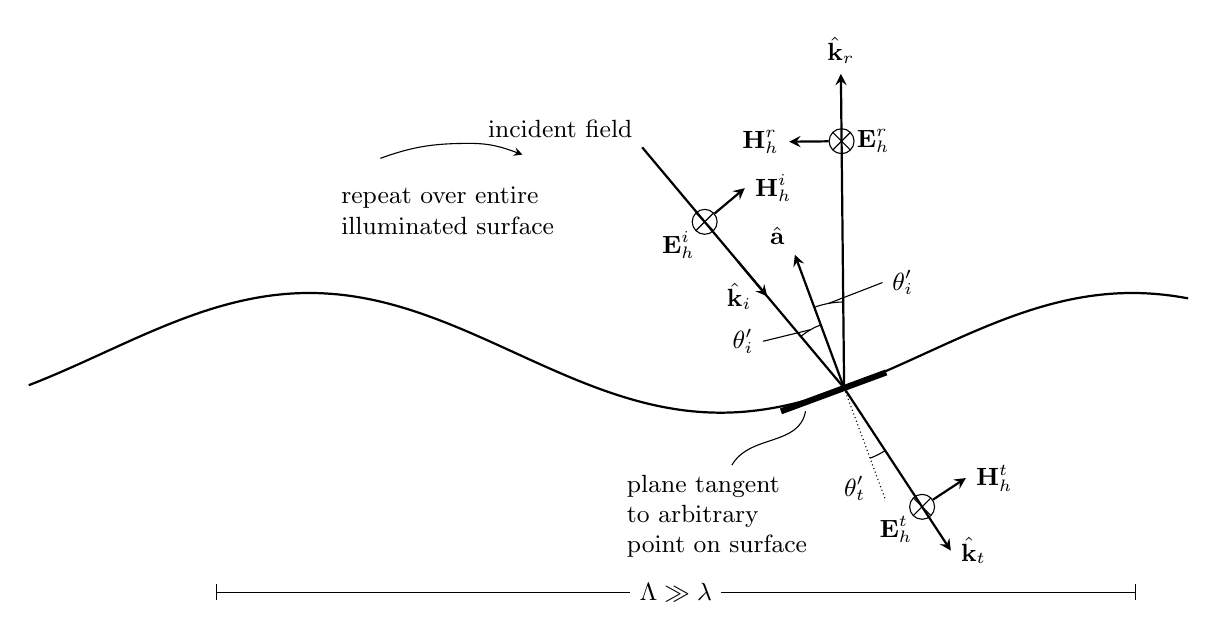
\begin{tikzpicture}[>=stealth, font=\small, scale=0.95,
		otimes/.style={circle, draw, inner sep=0pt, minimum size=9pt, path picture={
			\draw (path picture bounding box.north west) -- (path picture bounding box.south east)
				(path picture bounding box.south west) -- (path picture bounding box.north east);}}]
		\coordinate (P) at (10.9,-0.4702);
		% surface and tangent segment
		\draw[thick, domain=0:15.5, samples=200, smooth] plot (\x,{0.8*sin(deg(2*pi*(\x-1)/11))});
		\draw[line width=2.2pt] ($(P)+(200.29:0.9)$) -- ($(P)+(20.29:0.6)$);
		\draw ($(P)+(200.29:0.55)+(0,-0.12)$) to[out=-100,in=60] (9.4,-1.5);
		\node[anchor=north, align=left] at (9.2,-1.5) {plane tangent\\to arbitrary\\point on surface};
		% normal and its continuation
		\draw[->, thick] (P) -- ++(110.29:1.9) node[above left] {$\hat{\mathbf{a}}$};
		\draw[densely dotted] (P) -- ++(-69.71:1.6);
		% incident ray (from 125 deg), reflected (95.58 deg), transmitted (-59.96 deg)
		\draw[thick] ($(P)+(130:4.2)$) -- (P);
		\draw[->, thick] ($(P)+(130:2.2)$) -- ($(P)+(130:1.6)$) node[left, xshift=-2pt] {$\hat{\mathbf{k}}_i$};
		\draw[->, thick] (P) -- ++(90.59:4.2) node[above] {$\hat{\mathbf{k}}_r$};
		\draw[->, thick] (P) -- ++(-56.72:2.6) node[right] {$\hat{\mathbf{k}}_t$};
		% fields: incident
		\node[otimes] (ni) at ($(P)+(130:2.9)$) {};
		\node[below left] at (ni) {$\mathbf{E}_h^i$};
		\draw[->, thick] (ni) -- ++(40:0.7) node[right] {$\mathbf{H}_h^i$};
		\node[anchor=south east] at ($(P)+(130:4.2)$) {incident field};
		% reflected
		\node[otimes] (nr) at ($(P)+(90.59:3.3)$) {};
		\node[right=2pt] at (nr) {$\mathbf{E}_h^r$};
		\draw[->, thick] (nr) -- ++(180.59:0.7) node[left] {$\mathbf{H}_h^r$};
		% transmitted
		\node[otimes] (nt) at ($(P)+(-56.72:1.9)$) {};
		\node[below left] at (nt) {$\mathbf{E}_h^t$};
		\draw[->, thick] (nt) -- ++(33.28:0.7) node[right] {$\mathbf{H}_h^t$};
		% angles
		\draw ($(P)+(110.29:0.9)$) arc (110.29:130:0.9);
		\draw ($(P)+(120:0.9)$) -- ($(P)+(150:1.25)$) node[left] {$\theta_i'$};
		\draw ($(P)+(90.59:1.15)$) arc (90.59:110.29:1.15);
		\draw ($(P)+(100.4:1.15)$) -- ($(P)+(70:1.5)$) node[right] {$\theta_i'$};
		\draw ($(P)+(-69.71:1.0)$) arc (-69.71:-56.72:1.0);
		\node at ($(P)+(-84:1.35)$) {$\theta_t'$};
		% repeat label
		\node[align=left] at (5.6,1.9) {repeat over entire\\illuminated surface};
		\draw[->] (4.7,2.6) to[out=20,in=180] (5.9,2.8) to[out=0,in=160] (6.6,2.65);
		% scale bar
		\draw[|-|] (2.5,-3.2) -- (14.8,-3.2);
		\node[fill=white] at (8.65,-3.2) {$\Lambda \gg \lambda$};
	\end{tikzpicture}
	\caption{Kirchhoff (physical optics) approximation: at each point of a gently undulating surface, the incident wave is reflected and transmitted as at the infinite plane tangent to the surface, with local angles $\theta_i'$ and $\theta_t'$ measured from the local normal $\hat{\mathbf{a}}$. H polarization is shown.}
	\label{f:undulating}
\end{figure}
% NOTE: the caption is an added description.

\begin{itemize}
	\item We can calculate the scattered and transmitted fields just as we did for the case of a planar interface (because all we've done is approximate the undulating surface as a bunch of planar surfaces)
	\begin{itemize}
		% NOTE: added "(Lecture 5)".
		\item[$\Rightarrow$] the Fresnel reflection and transmission coefficients (Lecture 5) will play a role.
	\end{itemize}
\end{itemize}

\subsection{Backscatter toward the source}

\begin{itemize}
	\item To keep things simple and the course moving forward, we'll only consider the question of how much power is scattered back toward the source (as is the general case in ``active'' remote sensing).
	\item Again, skipping the details and simply noting that to do so, we need to consider the \underline{entire} scattered field $\Rightarrow$ integrate over the surface
	\begin{itemize}
		\item[$\rightarrow$] done by application of Green's theorem.
	\end{itemize}
	\item To get an analytical solution, it is necessary to make an assumption about the RMS height of the surface, $h$.
\end{itemize}

\subsubsection{Limit of small $h$, so that the surface slopes are shallow}

\begin{itemize}
	\item Allows for a reduced model for backscatter, commonly called the ``scalar approximation'' (pretty terrible name, but that's what we have).
	% NOTE: kept as handwritten ("Ulaby et al. (1986) Ch 12"), but the year or chapter may be off: in the U&L 2014
	% bibliography the surface-scattering volume is Vol. II, "Radar Remote Sensing and Surface Scattering and Emission
	% Theory" (Ulaby, Moore & Fung 1982), while the 1986 volume is Vol. III, "Volume Scattering and Emission Theory...".
	% Chapter numbers are not verifiable in either book.
	\item The ``scalar approximation'' expression for backscatter is pretty gnarly, and we won't repeat it here $\rightarrow$ see Ulaby et al.\ (1986), Ch.~12, for the expression and details of the derivation.
	% NOTE: handwritten reads "backscattered power will increase with roughness height and with decreasing wavelength
	% (i.e., steepening surface slope)"; the parenthetical moved to follow "roughness height", because at fixed ell the
	% slope scales with h (rms slope sqrt(2) h/ell for a Gaussian correlation function; U&L 2014, Eq. 10.10, p. 425;
	% van Zyl 2011, Eq. 5.1-8, p. 185) and does not depend on the EM wavelength.
	\item Key point is that shallow slopes allow for both coherent (specular) and incoherent (diffuse) scatter $\rightarrow$ in general, backscattered power will increase with roughness height (i.e., steepening surface slope) and with decreasing wavelength.
\end{itemize}

\subsubsection{Limit of large $h$ ($h \equiv$ RMS roughness height)}

\begin{itemize}
	\item Allows us to assume the gradient of the phase is negligible (``stationary phase approximation'').
	% NOTE: checked by derivation (python3): the stationary-phase (geometric optics) backscatter is
	% sigma^0 = pi |rho(0)|^2 sec^4(theta_i) p(tan theta_i, 0), with p the 2D Gaussian slope pdf of per-direction variance
	% -h^2 rho''(0) = 2 h^2/ell^2 (Gaussian correlation function; U&L 2014, Eqs. 10.9--10.10, p. 425), which gives
	% Eq. (e:go) with m = h/ell exactly. Equivalently, 4 m^2 = 4 h^2/ell^2 is the total mean-square slope s_g^2 of
	% van Zyl 2011, Eq. 5.1-8 (p. 185), and 2 m_rms^2 in terms of U&L's rms slope m_rms = sqrt(2) h/ell. With the
	% exponential correlation function the slopes are unbounded (van Zyl Eq. 5.1-9; U&L p. 428), so Eq. (e:go) with
	% m = h/ell assumes a Gaussian correlation function; added "(Gaussian correlation function)".
	\item It can be shown in this case (Gaussian correlation function) that
	\begin{equation}
		\label{e:go}
		\sigma_{pp}^0 = \frac{|\rho_p(0)|^2}{4m_s^2\cos^4\theta_i}\exp\left\{-\frac{\tan^2\theta_i}{4m_s^2}\right\},
	\end{equation}
	where
	\begin{itemize}
		\item $p = h$ or $v$ polarization;
		\item $m_s = h/\ell \equiv$ characteristic surface slope;
		% NOTE: added "(the Fresnel coefficient evaluated at theta_i = 0; not the correlation function of Eq. e:acf, for
		% which rho(0) = 1)", because the handwriting uses rho for both (master table D46).
		\item $\rho_p(0) = \rho(0) \equiv$ Fresnel reflection coefficient at normal incidence (the Fresnel coefficient evaluated at $\theta_i = 0$; not the correlation function of Eq.~\eqref{e:acf}, for which $\mathcal{C}(0) = 1$).
	\end{itemize}
	(Note: $\sigma_{hv}^0 = \sigma_{vh}^0 = 0$ in this model $\Rightarrow$ no depolarization.)
	% NOTE: added "gives Figure~\ref{f:go}".
	\item Plotting this expression for $\theta_i = 45^\circ$ and a range of slopes gives Figure~\ref{f:go}.
\end{itemize}

\begin{figure}[!htbp]
	\centering
	% Curve from Eq. (e:go) at theta_i = 45 deg: sigma^0/|rho(0)|^2 = exp[-1/(4 m^2)]/m^2 (cos^4 45 deg = 1/4), maximum 4/e
	% at m = 1/2 exactly (python3), as in the sketch (dashed line at m = 1/2). Ticks 0, 1/2, 1, 2 as handwritten.
	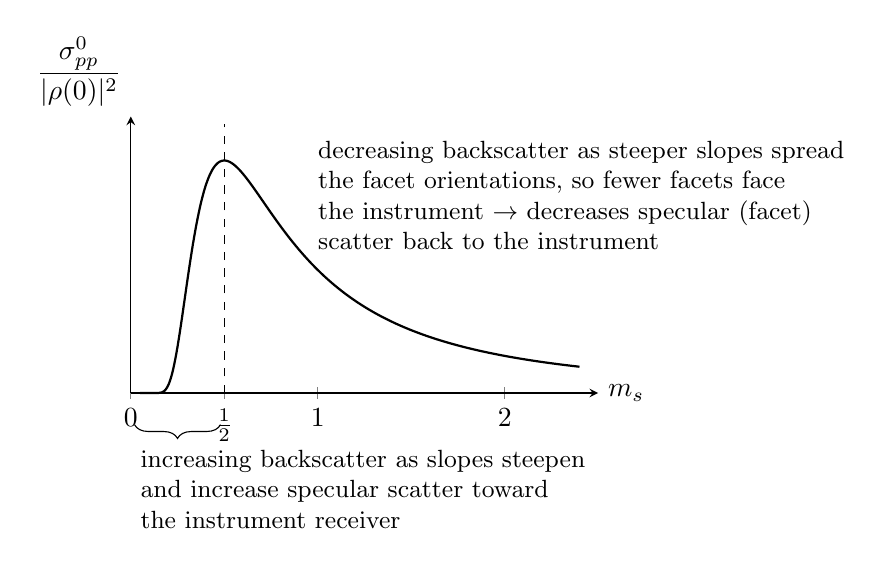
\begin{tikzpicture}
		\begin{axis}[
			width=0.62\textwidth, height=0.42\textwidth,
			axis lines=left, xmin=0, xmax=2.5, ymin=0, ymax=1.75,
			xtick={0,0.5,1,2}, xticklabels={$0$,$\frac12$,$1$,$2$}, ytick=\empty,
			xlabel={$m_s$}, ylabel={$\dfrac{\sigma_{pp}^0}{|\rho(0)|^2}$},
			ylabel style={rotate=-90},
			every axis x label/.style={at={(current axis.right of origin)},anchor=west},
			every axis y label/.style={at={(current axis.above origin)},anchor=south east},
			clip=false,
			]
			\addplot[dashed, thin] coordinates {(0.5,0) (0.5,1.7)};
			\addplot[thick, samples=400, domain=0.05:2.4] {exp(-1/(4*x^2))/x^2};
			\node[anchor=west, align=left, font=\small] at (axis cs:0.95,1.25) {decreasing backscatter as steeper slopes spread\\the facet orientations, so fewer facets face\\the instrument $\rightarrow$ decreases specular (facet)\\scatter back to the instrument};
			\draw[decorate, decoration={brace, mirror, amplitude=5pt}] (axis cs:0.02,-0.2) -- (axis cs:0.48,-0.2);
			\node[anchor=north west, align=left, font=\small] at (axis cs:0.0,-0.3) {increasing backscatter as slopes steepen\\and increase specular scatter toward\\the instrument receiver};
		\end{axis}
	\end{tikzpicture}
	\caption{Backscattering coefficient of Eq.~\eqref{e:go}, normalized by $|\rho(0)|^2$, versus the characteristic surface slope $m_s$ for $\theta_i = 45^\circ$.}
	\label{f:go}
\end{figure}
% NOTE: the caption is an added description. The handwritten annotation on the decreasing branch reads "decreasing
% backscatter as steeper terrain starts to shadow other terrain -> decreases specular (coherent) scatter back to
% instrument"; corrected because Eq. (e:go) contains no shadowing term: for m > 1/2 the backscatter falls because the
% slope pdf at the specular slope tan 45 deg = 1 decreases as the slope variance grows (derivation above; van Zyl
% 2011, p. 197: in this limit the scattering "is related to the number of surface facets that are oriented such that
% they reflect specularly in that direction"). "(coherent)" written "(facet)": in the backscatter direction at 45 deg
% there is no coherent component, which exists only near the specular direction (U&L 2014, Eqs. 5.115--5.117, p. 200);
% the facet reflections add incoherently.

\begin{itemize}
	\item The applicability of the model to natural terrain is limited due to the restrictions of the assumptions, but the intuition we build from the approach (simplifying assumptions) and the results (backscatter power is amplified for certain terrain) is valuable for more realistic scattering models.
\end{itemize}

%%%%%%%%%%%%%%%%%%%%%%%%%%%%%%%%%%%%%
% Symbols follow the master table in ../variables_master.tex; see it for flagged dual usages.
\clearpage
\section*{Variables}

Units are SI. Values are given for universal constants; ``typical'' values are representative, not definitive.

{\small
\renewcommand{\arraystretch}{1.25}
\begin{longtable}{>{$}l<{$} >{\raggedright\arraybackslash}p{0.37\textwidth} >{\raggedright\arraybackslash}p{0.15\textwidth} >{\raggedright\arraybackslash}p{0.24\textwidth}}
\hline
\textrm{Symbol} & Description & Units & Value \\
\hline
\endfirsthead
\hline
\textrm{Symbol} & Description & Units & Value \\
\hline
\endhead
\hline
\endfoot
\multicolumn{4}{l}{\emph{Constants and wavenumbers}} \\
j & imaginary unit, $j^2 = -1$ (time dependence $e^{j\omega t}$) & -- & -- \\
k & angular wavenumber in the medium above the surface & rad/m & $k_0 = 2\pi/\lambda$ for air \\
\lambda & wavelength (radar) & m & -- \\
d_\mathrm{ant} & largest dimension of the antenna (source) & m & far field: $R \ge 2d_\mathrm{ant}^2/\lambda$ \\
\multicolumn{4}{l}{\emph{Radar equation}} \\
R & distance (range); in the far field $R \gg \lambda$ & m & -- \\
R_t,\ R_r & distances from the transmit antenna to the scatterer and from the scatterer to the receiver & m & $R_t = R_r = R$ (same antenna) \\
P_t & transmit power & W & -- \\
G_t,\ G_r,\ G & gains of the transmit and receive antennas; common gain & dimensionless & $G_r = G_t = G$ (same antenna) \\
\mathcal{S}_s & power density at the scatterer (magnitude of the Poynting vector) & W/m$^2$ & $P_tG_t/(4\pi R_t^2)$ \\
A_{\mathrm{eff},s} & effective receiving area of the scatterer & m$^2$ & unknown \\
P_{rs} & total power received by the scatterer & W & $\mathcal{S}_sA_{\mathrm{eff},s}$ \\
f_a & fraction of power absorbed by the scatterer & dimensionless & $0$--$1$ \\
P_{ts} & power radiated by the scatterer & W & $P_{rs}(1 - f_a)$ \\
G_{ts} & gain of the scatterer in the direction of the receiver & dimensionless & unknown \\
\mathcal{S}_r & power density at the receiver & W/m$^2$ & -- \\
A_\mathrm{eff} & effective area of the receiving aperture & m$^2$ & $\lambda^2G_r/(4\pi)$ (lossless antenna) \\
P_r & power entering the receiver & W & -- \\
\sigma & radar (scattering) cross section, $A_{\mathrm{eff},s}(1 - f_a)G_{ts}$ & m$^2$ & -- \\
\sigma_{(n)},\ A_{(n)} & radar cross section of individual scatterer $n$ and its illuminated area & m$^2$ & -- \\
\sigma^0 & normalized radar cross section (``sigma-naught''), $\langle\sigma_{(n)}/A_{(n)}\rangle_n$ & dimensionless (m$^2$/m$^2$) & -- \\
p,\ q & polarization of the received and transmitted waves & -- & $h$ or $v$ \\
P_p^r,\ P_q^t & $p$-polarized received power; $q$-polarized transmit power & W & -- \\
\sigma_{pq}^0 & normalized radar cross section for receive/transmit polarizations $p$, $q$ & dimensionless & $\sigma_{hv}^0 = 0$ in Eq.~\eqref{e:go} \\
A & area illuminated (nominal area of illumination) & m$^2$ & -- \\
E_p^s,\ E_q^i & scattered ($p$-polarized) and incident ($q$-polarized) electric fields & V/m & -- \\
\Gamma_{pq} & reflectance, $|E_p^s|^2/|E_q^i|^2$ (depends on range, $\propto 1/R^2$) & dimensionless & -- \\
\multicolumn{4}{l}{\emph{Surface scattering}} \\
x,\ y,\ z & Cartesian coordinates & m & surface in the $x$--$y$ plane \\
\hat{\mathbf{k}}_i,\ \hat{\mathbf{k}}_r,\ \hat{\mathbf{k}}_t & propagation unit vectors of the incident, reflected, and transmitted waves & dimensionless & -- \\
\theta_i & angle of incidence & rad & -- \\
\multicolumn{4}{l}{\emph{Surface roughness}} \\
\xi(x,y) & local surface height & m & zero mean \\
h & RMS height, $\langle\xi^2\rangle^{1/2}$ & m & -- \\
x',\ y' & coordinates of a second point on the surface & m & -- \\
\mathcal{C}(r) & surface-height auto-correlation function & dimensionless & $\mathcal{C}(0) = 1$; $\mathcal{C}(\ell) = e^{-1}$ \\
r & horizontal separation between two surface points & m & -- \\
\rho & Fresnel reflection coefficient of a planar interface (Lectures 4--5) & dimensionless & -- \\
\Gamma & reflectivity of an infinite planar interface, $|\rho|^2$ & dimensionless & $0$--$1$ \\
\ell & correlation length & m & -- \\
W & roughness spectrum & m$^2$ & -- \\
k_x,\ k_y & spectral wavenumbers of the surface roughness & rad/m & backscatter: $(-2k\sin\theta_i, 0)$ \\
u,\ v & separations in $x$ and $y$ (lags) & m & -- \\
\theta_s & scattering angle & rad & $\theta_i$ in backscatter \\
\phi_s & scattering azimuth & rad & $\pi$ in backscatter \\
\multicolumn{4}{l}{\emph{Undulating surface}} \\
\Lambda & wavelength of the surface undulations & m & $\Lambda \gg \lambda$ \\
\hat{\mathbf{a}} & local unit normal to the surface & dimensionless & -- \\
\theta_i',\ \theta_t' & local angles of incidence and transmission (from $\hat{\mathbf{a}}$) & rad & -- \\
\mathbf{E}_h^i,\ \mathbf{H}_h^i,\ \ldots & H-polarized incident, reflected, and transmitted fields & V/m; A/m & -- \\
m_s & characteristic surface slope, $h/\ell$ (Ulaby \& Long's rms slope is $\sqrt{2}\,h/\ell$) & dimensionless & peak backscatter at $m_s = 1/2$ for $\theta_i = 45^\circ$ \\
\rho_p(0) & Fresnel reflection coefficient at normal incidence ($p$ polarization) & dimensionless & -- \\
\sigma_{pp}^0 & co-polarized normalized radar cross section & dimensionless & -- \\
\end{longtable}
}

\end{document}
